\documentclass[hidelinks,12pt]{article}
\usepackage[a4paper,width=150mm,top=25mm,bottom=25mm]{geometry}
\usepackage[utf8]{inputenc}
\usepackage{graphicx}
\usepackage{lipsum}
\usepackage{amssymb}
\usepackage{apacite}
\usepackage{natbib}
\usepackage{hyperref}
\usepackage{float}
\usepackage{ragged2e}
\usepackage[font={footnotesize,bf}]{caption}
\usepackage[nottoc,numbib]{tocbibind}
\usepackage{multirow}
\usepackage{placeins}
\usepackage{booktabs}
\usepackage{hyperref}
\hypersetup{
    colorlinks=true,
    linkcolor=blue,
    filecolor=magenta,      
    urlcolor=cyan,
    pdftitle={Overleaf Example},
    pdfpagemode=FullScreen,
    }
\renewcommand{\thesubsection}{\thesection.\alph{subsection}}

\linespread{1.5}

\begin{document}

\begin{titlepage}
    \begin{center}
        \vspace*{1cm}
        
        
        % \vfill
        
        \large
        \textbf{Big Data Asset Pricing \\ Exercise 4: Hig-Dimensional Return Predictions}
            
        
        \normalsize
        Seyyed Morteza Aghajanzadeh \\
        Department of Finance \\
        Stockholm School of Economics
        
        \vfill
        \normalsize
        \justifying
        \noindent
        \textbf{Statement:} I certify with my signature that I have solved the exercise according to the Code of Professional Conduct and Ethics. 
        For example, I have not plagiarized others, but, instead, solved the exercise myself (possibly with allowed collaboration with other students), and I have referenced my sources appropriately.

        \vfill
        
        \vspace{0.8cm}
            
        
        \vspace{0.8cm}
        \normalsize
        \centering
        2024-01
            
    \end{center}
\end{titlepage}

\section{}

\begin{figure}[htbp]
    \centering
    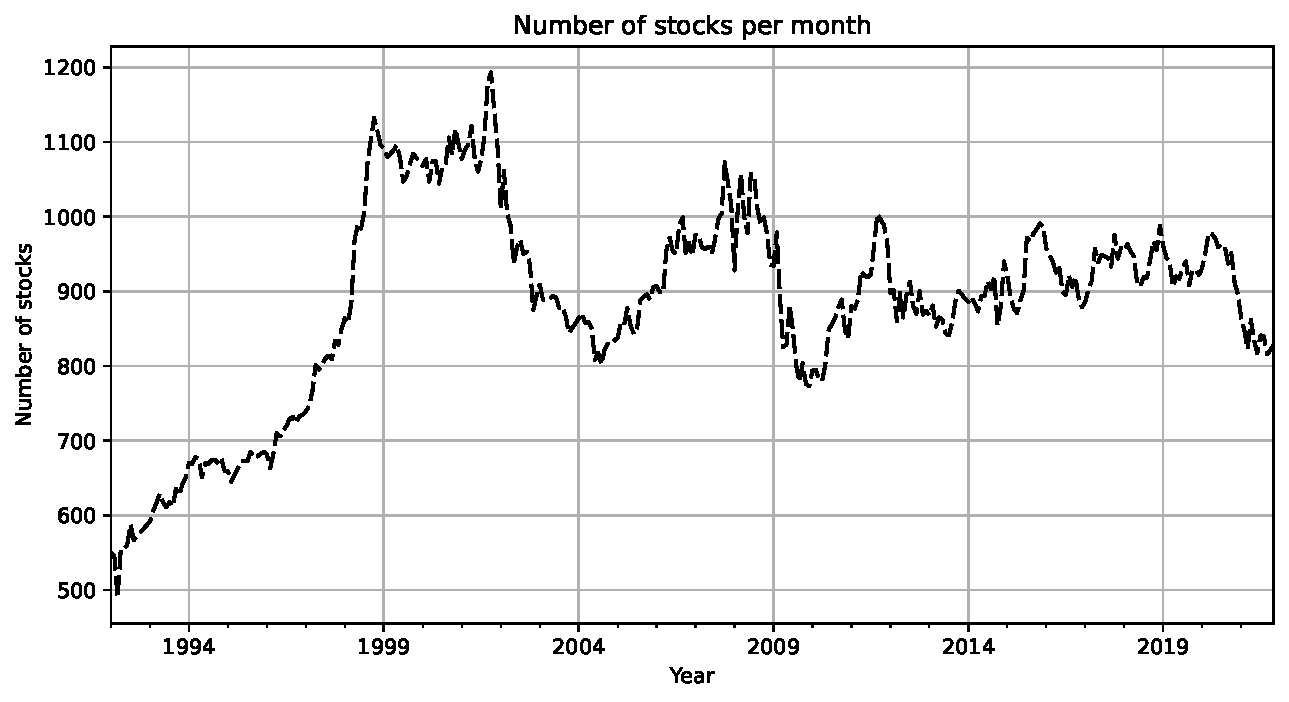
\includegraphics[width=.95\textwidth]{out/1.pdf}
\end{figure}

\FloatBarrier

\section{}
\subsection{}
\begin{table}[htbp]
    \centering
    \caption{The table shows the results of the Fama-Macbeth regression.}
    \resizebox{.9\textwidth}{!}{\begin{tabular}{lcccccc}
\toprule
                        & \textbf{Parameter} & \textbf{Std. Err.} & \textbf{T-stat} & \textbf{P-value} & \textbf{Lower CI} & \textbf{Upper CI}  \\
\midrule
\textbf{be\_me}         &       0.0282       &       0.0261       &      1.0822     &      0.2792      &      -0.0229      &       0.0794       \\
\textbf{ret\_12\_1}     &      -0.0231       &       0.0208       &     -1.1070     &      0.2683      &      -0.0639      &       0.0178       \\
\textbf{market\_equity} &      -0.0490       &       0.0260       &     -1.8887     &      0.0589      &      -0.0999      &       0.0019       \\
\bottomrule
\end{tabular}
%\caption{Parameter Estimates}}
\end{table}

\subsection{}
\begin{figure}[htbp]
    \centering
    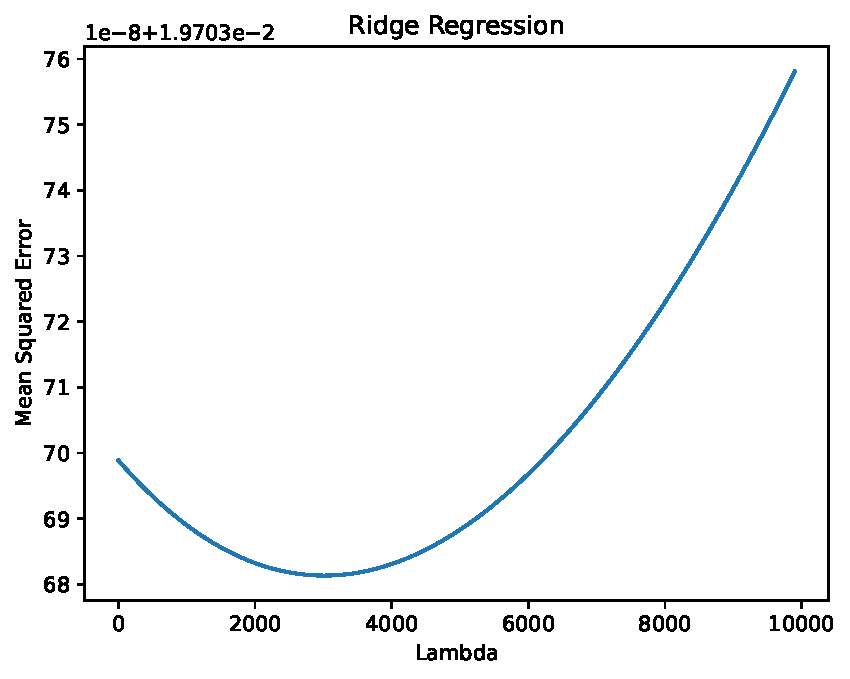
\includegraphics[width=.95\textwidth]{out/2_2.pdf}
\end{figure}

\FloatBarrier
\subsection{}
\begin{figure}[htbp]
    \centering
    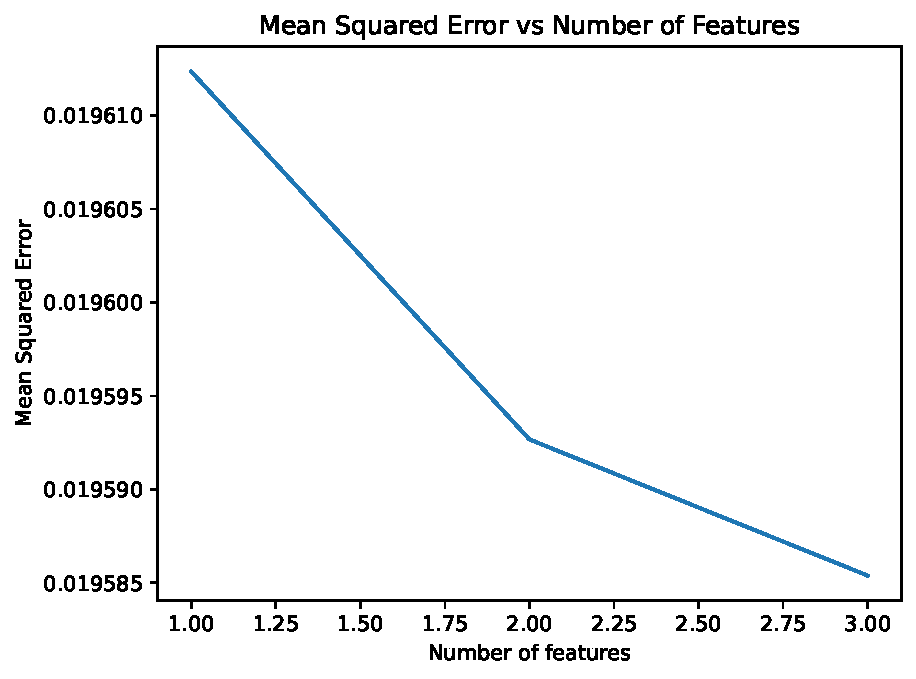
\includegraphics[width=.75\textwidth]{out/2_3_1.pdf}
    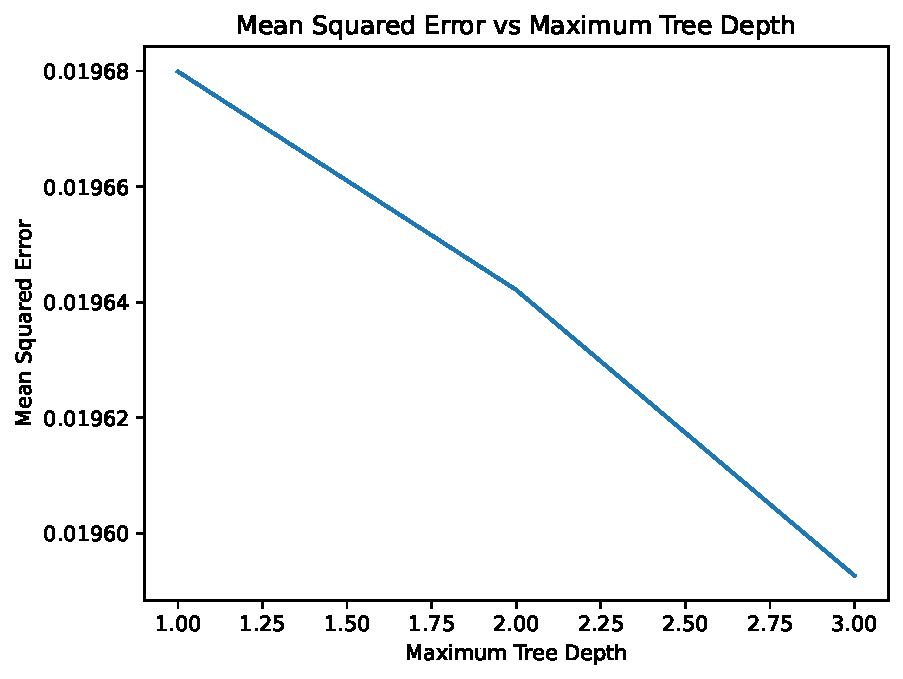
\includegraphics[width=.75\textwidth]{out/2_3_2.pdf}
    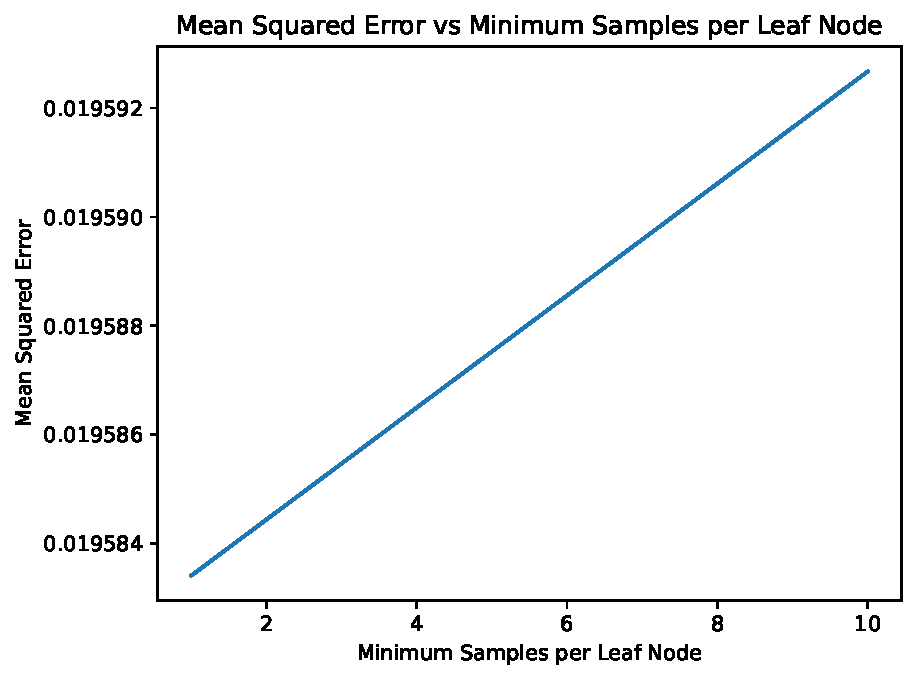
\includegraphics[width=.75\textwidth]{out/2_3_3.pdf}
\end{figure}


\FloatBarrier

\section{}
\begin{table}[htbp]
    \centering
    \caption{}
    \resizebox{!}{!}{\begin{tabular}{cc}
\hline
  Model  &  In-sample R2  \\
\hline
 Model A &     0.0012     \\
 Model B &     0.0010     \\
 Model C &     0.0010     \\
\hline
\end{tabular}}
\end{table}

\section{}

\begin{figure}[htbp]
    \centering
    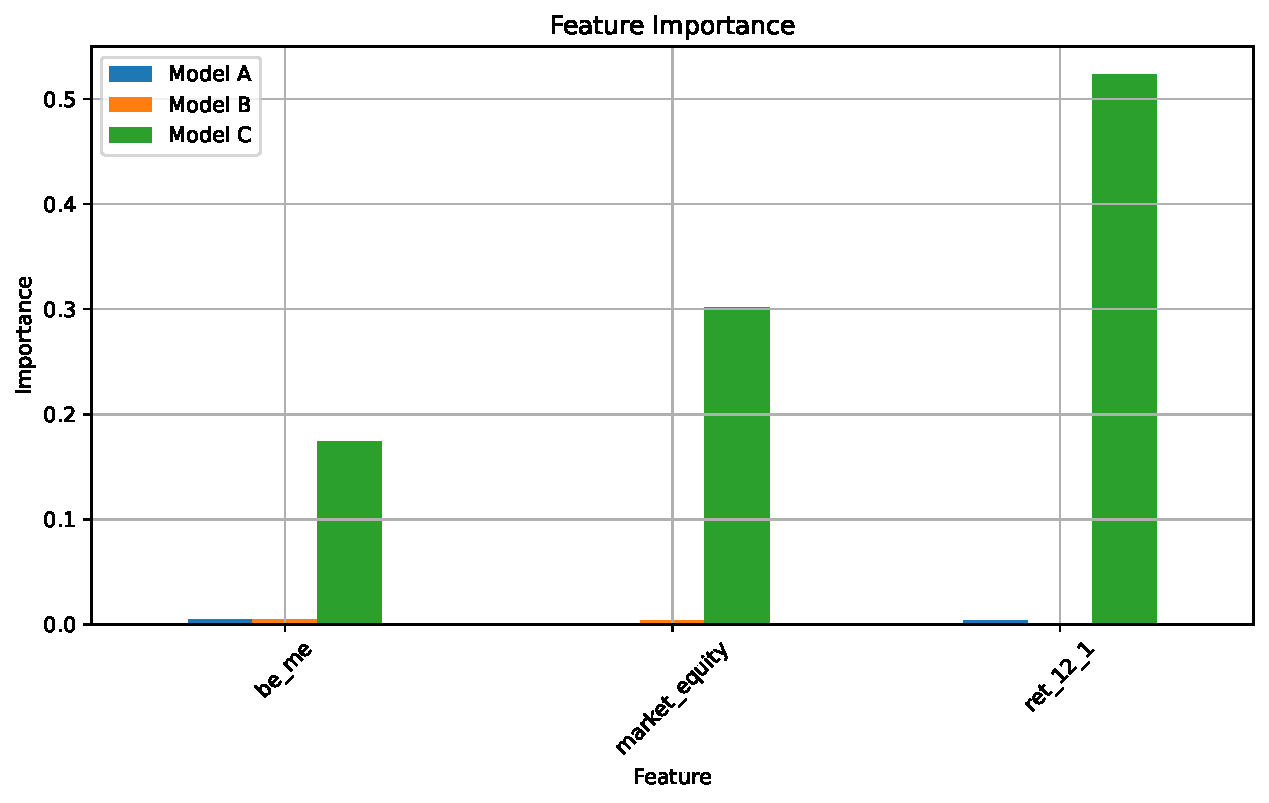
\includegraphics[width=.75\textwidth]{out/4.pdf}
\end{figure}

\section{}
\subsection{}
\begin{table}[htbp]
    \centering
    \caption{}
    \resizebox{!}{!}{\begin{tabular}{cc}
\hline
  Model  &  Out-sample R2  \\
\hline
 Model A &     0.2471      \\
 Model B &     0.0010      \\
 Model C &     0.0010      \\
\hline
\end{tabular}}
\end{table}

\subsection{}
\begin{table}[htbp]
    \centering
    \caption{}
    \resizebox{!}{!}{\begin{tabular}{lcccccc}
\toprule
$r_i - r_f$ & t-stat & $\alpha$ & $t(\alpha)$ & Sharpe Ratio & Information Ratio \\
\midrule
-0.0052 & -0.1389 & -0.0043 & -1.2000 & -0.1389 & -0.1184 \\
0.5403 & 0.0810 & 0.5804 & 0.9003 & 0.0810 & 0.0872 \\
0.0803 & 0.0414 & 0.0865 & 0.4852 & 0.0414 & 0.0447 \\
\bottomrule
\end{tabular}
}
\end{table}




\appendix

\section*{Appendix}

Here you can find the python code that I used to solve the exercise. \href{https://github.com/mortezaaghajanzadeh/BDAP/tree/main/Assignments/Assignment4}{Link to the GitHub repository.}

\end{document}